\chapter{Admittance Control}
In this chapter, we will explain why we use the cooperative aerial manipulation system to help solve the secondary requirements,. we will introduce how to integrated the impedance control and admittance control together, as well as how can we realize it in the multi-link aerial robot. Finally, the integrated hybrid impedance-admittance control will be introduced and present in the experiments by using the 3D multi-link aerial robot DRAGON, and show it can imitate the traditional cooperative aerial manipulation systems and help to solve the secondary requirements.

%%%%%%%%%%%%%%%%%%%%%%%%%%%%%%%%%%%%%%%%%%%%%%%%%%%%%%%%%%%%%%%%%%%%%%%%%%%%%%%%
\section{Framework Overview}

\begin{figure}[h]
    \centering
    % \parbox{3in}
    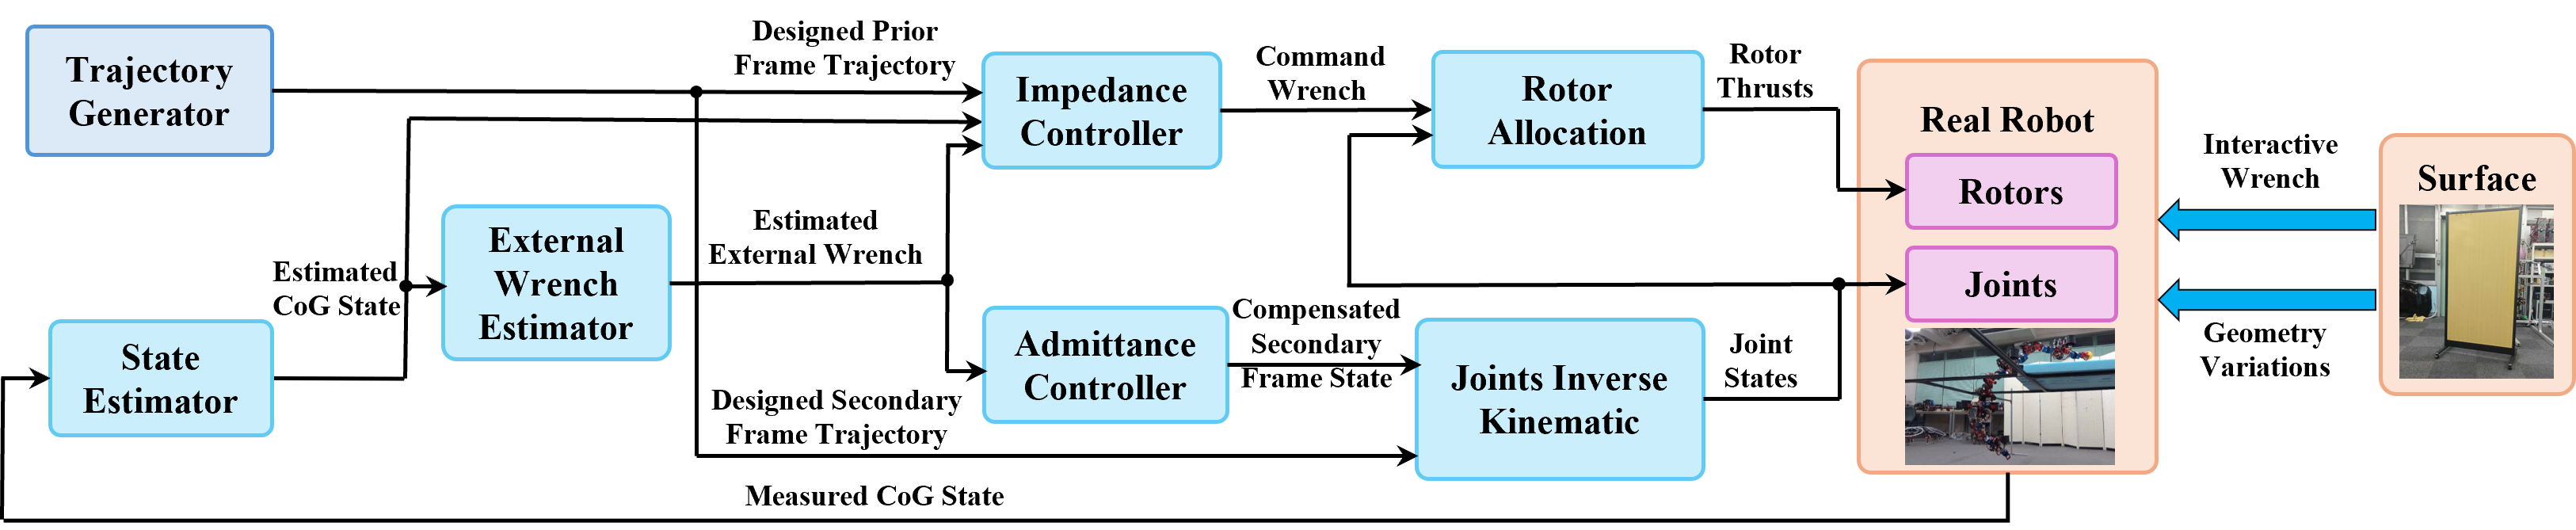
\includegraphics[trim={0cm 0.3cm 0cm 0cm}, clip,width=\linewidth]{figures/chapter4/framework_dragon.png}
    \caption{Block diagram of the hybrid impedance-admittance control framework. Inputs for the admittance controller consist of the estimated external wrench. Inputs for the impedance controller include the state reference, estimated CoG state, and estimated external wrench.}
    \label{fig:framework_dragon}
    \vspace{-5mm}
\end{figure}

As illustrated in Fig.~\ref{fig:framework_dragon}, impedance control manages the overall state of one reference point on the aerial robot, while admittance control is applied to regulate the distance between the end effector and the reference point, resulting in adjustments of the joint angles. Since variations in joint angles modify the robot's configuration and thus influence the thrust allocation, this dependency is taken into account in the thrust computation.
The propose of we control two points on multi-link aerial robot is to imitate double aerial robot cooperation. Compared to the swarm aerial manipulation, single aerial robot can provide more stability. It is more good to guarantee the distance between the two points.
We consider the two selected frame on the dragon as the adjusting frame. We can consider one of them as a prior frame and the other as the secondary frame. The pose of the prior frame is completely controlled by the impedance control, and the pose of the secondary frame related to the prior frame is controlled by the designed trajectory and admittance control. In this framework, the impedance control is used for stably control the prior frame to follow its trajectory, while the admittance control is used for adjust the unmodeled geometric part that the secondary frame may face to. Depending to task requirement, there will be a lot of choices. 
Overall, the hybrid controller added in dragon is to imitate the double drones cooperation aerial manipulation by the single aerial robot.

%%%%%%%%%%%%%%%%%%%%%%%%%%%%%%%%%%%%%%%%%%%%%%%%%%%%%%%%%%%%%%%%%%%%%%%%%%%%%%%%
\section{Impedance control mode setup}
If we what to control the prior frame, we need to do frame transformation to get the error values used for impedance control. Usually, there are three important frames in the aerial robot: CoG frame, end effector frame and base link frame. Due to some kind of symmetry, there is no fundamental difference between the end effector frame and the base link frame. The reason why we set such kind of mode is to follow the kinematic modeling of the multi-link structure.
In real world experience, the meaning we use those three frames are different: The CoG frame can be considered as the overall state of the whole multi-link aerial robot, and it is very convenient to calculate because the command wrench needed to be calculated in the CoG frame. So if the task requires to guarantee the overall pose of the aerial robot, the CoG centric mode can be used. However, due to the CoG point is usually in the air for the special structure of the multi-link aerial robot, it usually lacks certain meaning to control this frame in the air. On the other hand, the end effector frame and the base link frame have different meaning. They are the head and rear end of the whole serial link structure, therefore can be used as the contact point. Meanwhile, other complicated requirements can be put forward. for example, we can use the end effector as the contact point to the surface, and used the base link to mount a camera, radar or other sensor. Or we can access a power cable in the base link. At this situation, the pose of the base link is also need to be consider, but it is not as important as the contact point. 
So in this thesis, we will choose the end effector frame as the prior frame and the base link frame as the secondary frame.


We only change the error in the impedance equations \ref{eq:imp cmd for trans2} and \ref{eq:imp cmd for rot2}
\subsection{CoG centric mode}
In the CoG centric mode (short as cog-centric), the errors are defined as usual
\begin{subequations}
\label{eq:error cog mode}
\begin{align}
    {\boldsymbol{e}_p}&={^W\!\boldsymbol{p}}-{^W\!\boldsymbol{p}_{ref}}, \\[2pt]
    {\boldsymbol{e}_v}&={^W\!\dot{\boldsymbol{p}}}-{^W\!\dot{\boldsymbol{p}}_{ref}}, \\[2pt]
    {\boldsymbol{e}_R}&=\frac{1}{2}({^W\!\boldsymbol{R}^{\mathrm{T}}_{C,ref}}{^W\!\boldsymbol{R}_{C}}-{^W\!\boldsymbol{R}^{\mathrm{T}}_{C}}{^W\!\boldsymbol{R}_{C,ref}})^\vee, \\[2pt]
    {\boldsymbol{e}_\omega}&={^C\!\boldsymbol{\omega}}-{^W\!\boldsymbol{R}^{\mathrm{T}}_{C}}{^W\!\boldsymbol{\omega}}_{ref},
\end{align}
\end{subequations}
after calculated the command wrench in the CoG frame, the value can be directly allocated to the rotors.
\subsection{end effector centric mode}
In the end effector centric mode (short as ee-centric).
The rotational impedance control is considered in the $\{E\}$ frame.

\begin{equation}
\label{eq:impedance ee}
{\boldsymbol{I}_{d}}{^C\!\dot{\boldsymbol{\omega}}}+{\boldsymbol{C}_{rd}}{\boldsymbol{e}_\omega}+{\boldsymbol{K}_{rd}}{\boldsymbol{e}_R}={^E\!\boldsymbol{\tilde{\tau}}_{ext}},
\end{equation}

The errors are defined as
\begin{subequations}
\label{eq:error ee mode}
\begin{align}
    {\boldsymbol{e}_p}&={^W\!\boldsymbol{p}} + ^W\!\!R_C{^C\!\boldsymbol{p}_E}-{^W\!\boldsymbol{p}_{ref}}, \\[2pt]
    {\boldsymbol{e}_v}&={^W\!\dot{\boldsymbol{p}}}+{}^C\boldsymbol{\omega}^\wedge{}^C\boldsymbol{p}_E-{^W\!\dot{\boldsymbol{p}}_{ref}}, \\[2pt]
    {\boldsymbol{e}_R}&=\frac{1}{2}({^W\!\boldsymbol{R}^{\mathrm{T}}_{C,ref}}{^W\!\boldsymbol{R}_{C}}{^C\!\boldsymbol{R}_{E}}-({^W\!\boldsymbol{R}_{C}}{^C\!\boldsymbol{R}_{E})^{\mathrm{T}}}{^W\!\boldsymbol{R}_{C,ref}})^\vee, \\[2pt]
    {\boldsymbol{e}_\omega}&={^C\!\boldsymbol{R}^{\mathrm{T}}_E{}^C\!\boldsymbol{\omega}}-{^C\!\boldsymbol{R}^{\mathrm{T}}_E {}^W\!\boldsymbol{R}^{\mathrm{T}}_{C}}{^W\!\boldsymbol{\omega}}_{ref},
\end{align}
\end{subequations} 
where we use the wedge-operator $^\wedge$ to transform a vector into a skew symmetric matrix.
Note that here we consider the joint variation is small enough in a control period, so we ignore some terms.
TODO: think about this part. Is the equation correct?

The original point of the end effector frame to realize the impedance behavior in the air, 

\begin{equation}
\label{eq:imp cmd for trans2}
    {^W\!\boldsymbol{f}_{cmd}}=(m\boldsymbol{M}^{-1}_d-\boldsymbol{E}_3){^W\!\boldsymbol{\tilde{f}}_{ext}}-m(\tilde{\boldsymbol{C}}_{td}{\boldsymbol{e}_v}+{\tilde{\boldsymbol{K}}_{td}}{\boldsymbol{e}_p})+m\boldsymbol{g}.
\end{equation}

\begin{equation}
\label{eq:imp cmd for rot2}
    {^{C}\boldsymbol{\tau}_{cmd}}=(\boldsymbol{I}(^C\boldsymbol{R}_E\boldsymbol{I}_d)^{-1}-\boldsymbol{E}_3){^{C}}\boldsymbol{\tilde{\tau}}_{ext}-\boldsymbol{I}^C\boldsymbol{R}_E^{-1}(\tilde{\boldsymbol{C}}_{rd}{\boldsymbol{e}_\omega}+\tilde{\boldsymbol{K}}_{rd}{\boldsymbol{e}_\alpha})+^C\boldsymbol{R}_E^{-1}(^C\!\boldsymbol{p}_E^\wedge{}^C\boldsymbol{\tilde{f}}_{ext})
    +{^{C}\boldsymbol{\omega}} \times \boldsymbol{I}{^{C}\boldsymbol{\omega}}.
\end{equation}

\subsection{base effector centric mode}
In the base effector centric mode (short as be-centric), the errors are defined as
\begin{subequations}
\label{eq:error be mode}
\begin{align}
    {\boldsymbol{e}_p}&={^W\!\boldsymbol{p}} + ^W\!\!R_C{^C\!\boldsymbol{p}_B}-{^W\!\boldsymbol{p}_{ref}}, \\[2pt]
    {\boldsymbol{e}_v}&={^W\!\dot{\boldsymbol{p}}}-{^W\!\dot{\boldsymbol{p}}_{ref}}, \\[2pt]
    {\boldsymbol{e}_R}&=\frac{1}{2}({^W\!\boldsymbol{R}^{\mathrm{T}}_{C,ref}}{^W\!\boldsymbol{R}_{C}}{^C\!\boldsymbol{R}_{B}}-({^W\!\boldsymbol{R}_{C}}{^C\!\boldsymbol{R}_{B})^{\mathrm{T}}}{^W\!\boldsymbol{R}_{C,ref}})^\vee, \\[2pt]
    {\boldsymbol{e}_\omega}&={^C\!\boldsymbol{\omega}}-{^W\!\boldsymbol{R}^{\mathrm{T}}_{C}}{^W\!\boldsymbol{\omega}}_{ref},
\end{align}
\end{subequations}
If we what to use the base link to do something, we can choose this mode.

As shown in Fig.~\ref{fig:admittance_changing}, the dragon choose different modes.
\begin{figure}[h]
    \centering
    % \parbox{3in}
    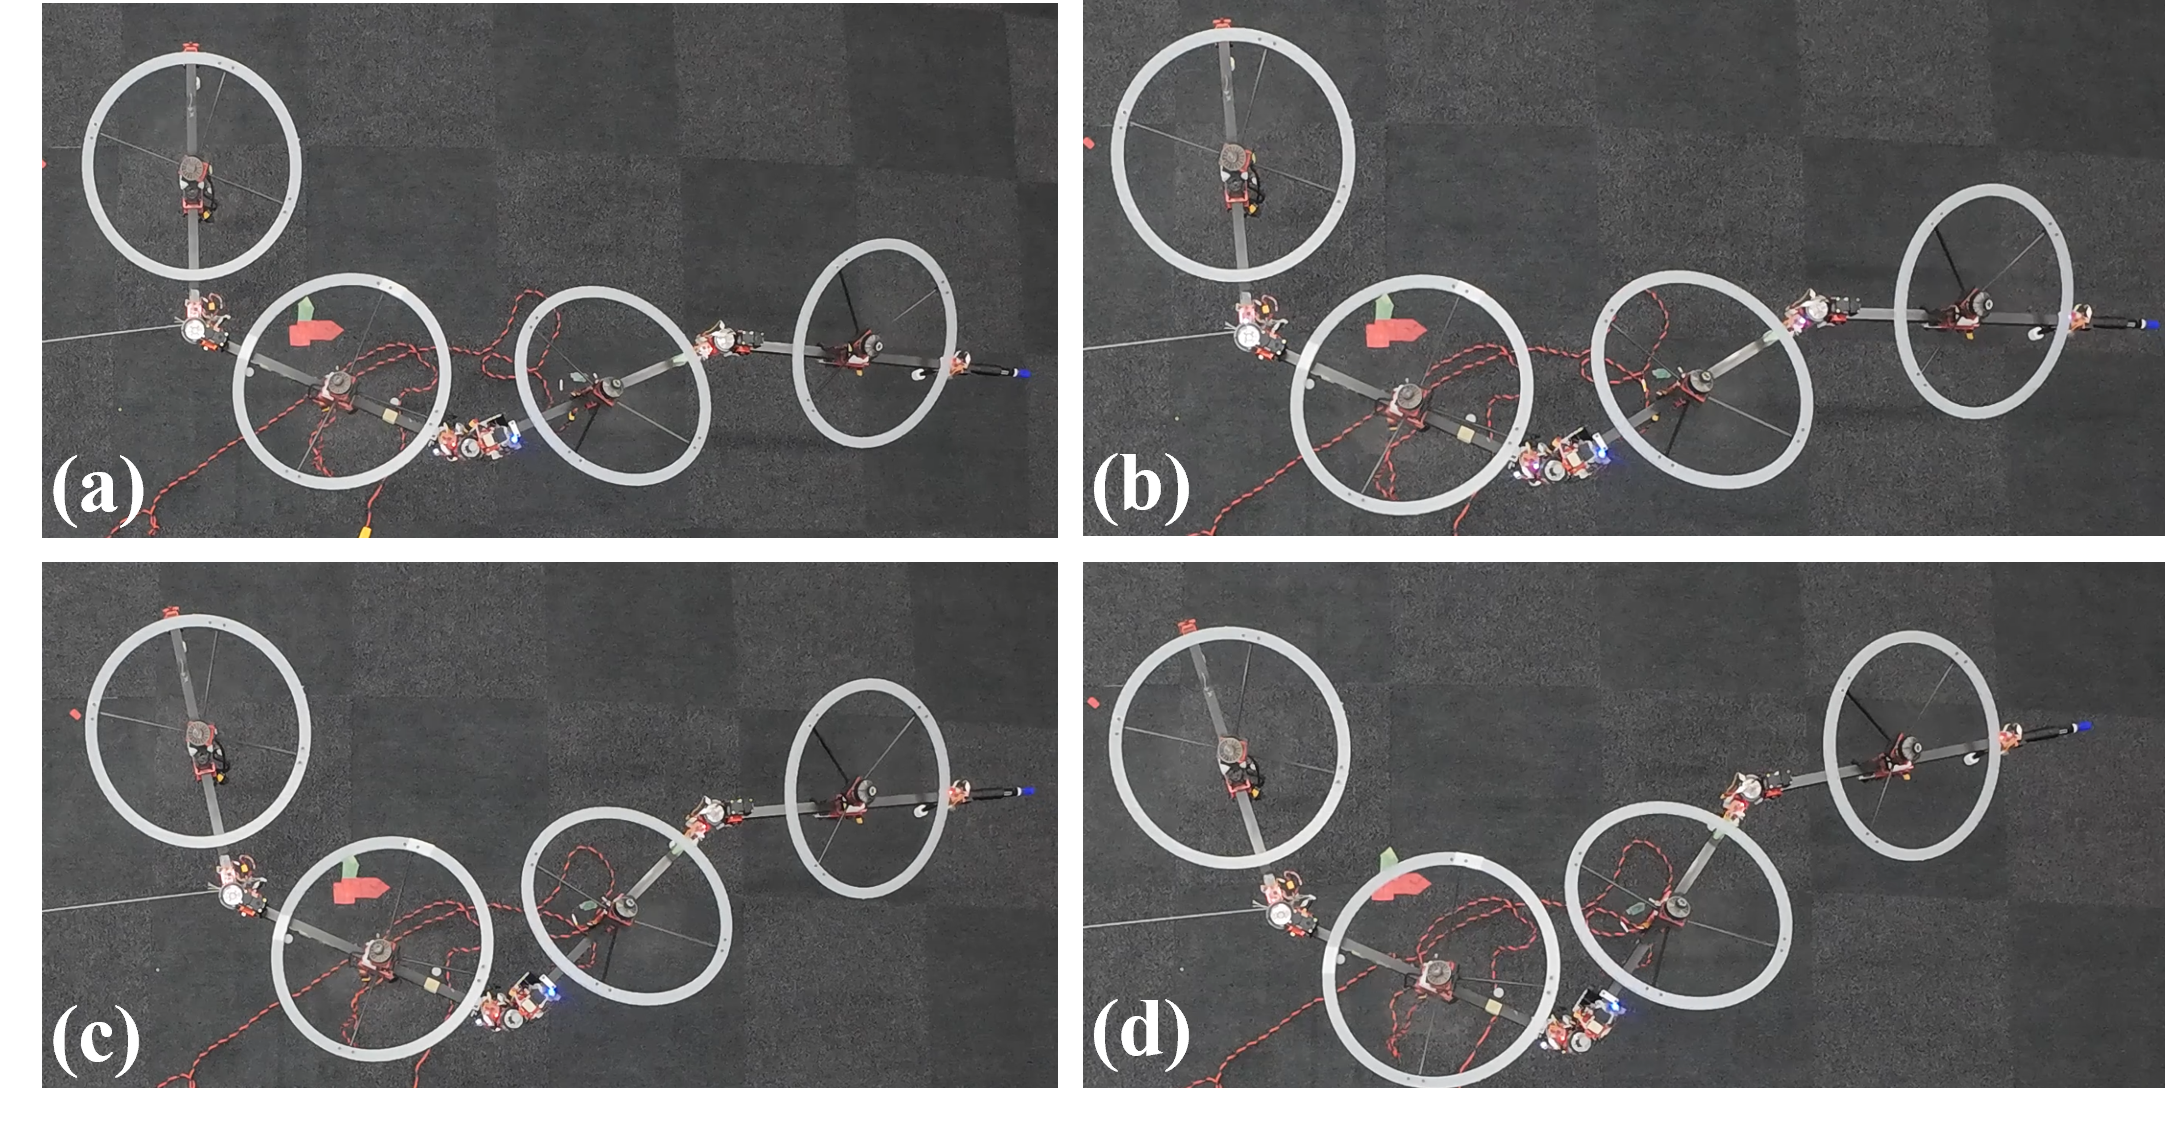
\includegraphics[trim={0cm 0.3cm 0cm 0cm},clip,width=\linewidth]{figures/chapter3/admittance_changing.png}
    \caption{Admittance changing.}
    \label{fig:admittance_changing}
    \vspace{-5mm}
\end{figure}

% %%%%%%%%%%%%%%%%%%%%%%%%%%%%%%%%%%%%%%%%%%%%%%%%%%%%%%%%%%%%%%%%%%%%%%%%%%%%%%%%
% \section{bb-centric/ee-centric in Impedance control}
% \subsection{why we need be-centric/ee-centric}
% \subsection{special setup for impedance control}
% Because the calculated wrench are defined in frame E or frame B, we need to transform them into CoG frame.
%%%%%%%%%%%%%%%%%%%%%%%%%%%%%%%%%%%%%%%%%%%%%%%%%%%%%%%%%%%%%%%%%%%%%%%%%%%%%%%%
\section{validation on Dragon}
\subsection{Impedance control on Dragon}
After that, the thrust and the gimbal angle can be set.
We need to get the command wrench of the aerial robot
\begin{equation}
\label{eq:command wrench dragon}
^C\mathbf{w}_{cmd}=\begin{pmatrix}
^C\!\boldsymbol{f}_{cmd} \\
^C\!\boldsymbol{\tau}_{cmd}
\end{pmatrix},
\end{equation}
here $^C\mathbf{w}_{cmd}$ is the command wrench in frame $\{C\}$.
Because dragon is the overactuated system, the command wrench can be achieve by its rotors simultaneously(if we ignore the servo response time). Therefore, after gaining the command wrench in $\{C\}$, we can used the equation () to calculated the rotor thrusts and gimbal servo angles.
% \begin{equation}
% \begin{aligned}
% \min_{\lambda,\,\theta,\,\phi} \quad & \|\boldsymbol{\lambda}\|^2 \\
% \mathrm{s.t.} \quad & ^C\mathbf{w}_{cmd} = \boldsymbol{Q}(\theta,\phi)\boldsymbol{\lambda}
% \end{aligned}
% \end{equation}
\subsection{Admittance control on Dragon}
Here the distance are consider as the distance between two selected frames. Usually, we will choose the distance between the end effector and base link as the admittance position. In detail, the distance $r$ is considered as the position of the original point of $\{E\}$ frame respect to the $\{B\}$ frame. 
$r = ^B\boldsymbol{p}_{BE}$ 
The distance influenced by the admittance control is  

We then employ a discrete-time difference method to compute the distance $\boldsymbol{r}$ at each time step, denoted as $\boldsymbol{r}[k]$. The corresponding acceleration is calculated as: 
\begin{equation}
\label{eq:difference method1}
\boldsymbol{\ddot{r}}[k]=\boldsymbol{M}^{-1}_a(({\boldsymbol{\tilde{f}}_{ext}}-\boldsymbol{f}_{ref})-\boldsymbol{K}_a(\boldsymbol{r}_{ref}-\boldsymbol{r}[k-1])+\boldsymbol{C}_a\boldsymbol{\dot{r}}[k-1]).
\end{equation}
Using this acceleration, the velocity and position can be updated iteratively according to:
\begin{subequations}
\label{eq:difference method2}
\begin{align}
\boldsymbol{\dot{r}}[k]&=\boldsymbol{\dot{r}}[k-1]+\boldsymbol{\ddot{r}}[k]\Delta t, \\[2pt]
\boldsymbol{r}[k]&=\boldsymbol{r}[k-1]+\boldsymbol{\dot{r}}[k]\Delta t,
\end{align}
\end{subequations}
where $\Delta t$ is the control period.



\subsection{Inverse Kinematics on Dragon}
In order to realize two trajectory in the air, we need to use inverse kinematics to get the joint angles of dragon. The prior trajectory is followed by the prior frame under impedance control. Depending the task requirements, we can calculated the relative transformation between the prior trajectory and the secondary trajectory, and regard it as the design position. For convenience, we only regard the transform from the $\{B\}$ frame to the $\{E\}$ frame, and represent it in the $\{B\}$ frame. The other part is the admittance distance. Therefore, we have to parts for theoretical position and unmodeled position compensation. As the following equation shows:


\begin{equation}
\label{eq:IK distance dragon}
\boldsymbol{r}_s = \boldsymbol{r}_{d} + \boldsymbol{r},
\end{equation}

here $\boldsymbol{r}_s$ means the real position of the end-effector in frame $\{B\}$. 
If we control the distance between the end effector frame and the base link frame, there will be six joints between them, which means the IK process can be considered as solve the IK problem in a six-dof robotic arms. Transparently, except some singular points, most of the pose can be reach by the serial link structure.

\begin{equation}
\label{eq:IK dragon}
\boldsymbol{q} = IK(^ER_{B,ref},\boldsymbol{r}_s),
\end{equation}
here the $^ER_{B,ref}$ is the desired rotation matrix from frame $\{B\}$ to frame $\{E\}$.
After we design the trajectory and the position error of admittance control. We calculate the joint angles. Finally, we will get the joint angles by inverse kinematics.
In theory, there will be more limitation. We need to consider whether the joints can execute the command, and the aerial robot may lose controllability at some configurations. In this work, we only attempt those configurations that successfully executed in simulation. The influence process hope to be solved in the future work.

As shown in Fig.~\ref{fig:admittance_changing}, the multi-link structure can follow the trajectory under inverse kinematics.
\begin{figure}[h]
    \centering
    % \parbox{3in}
    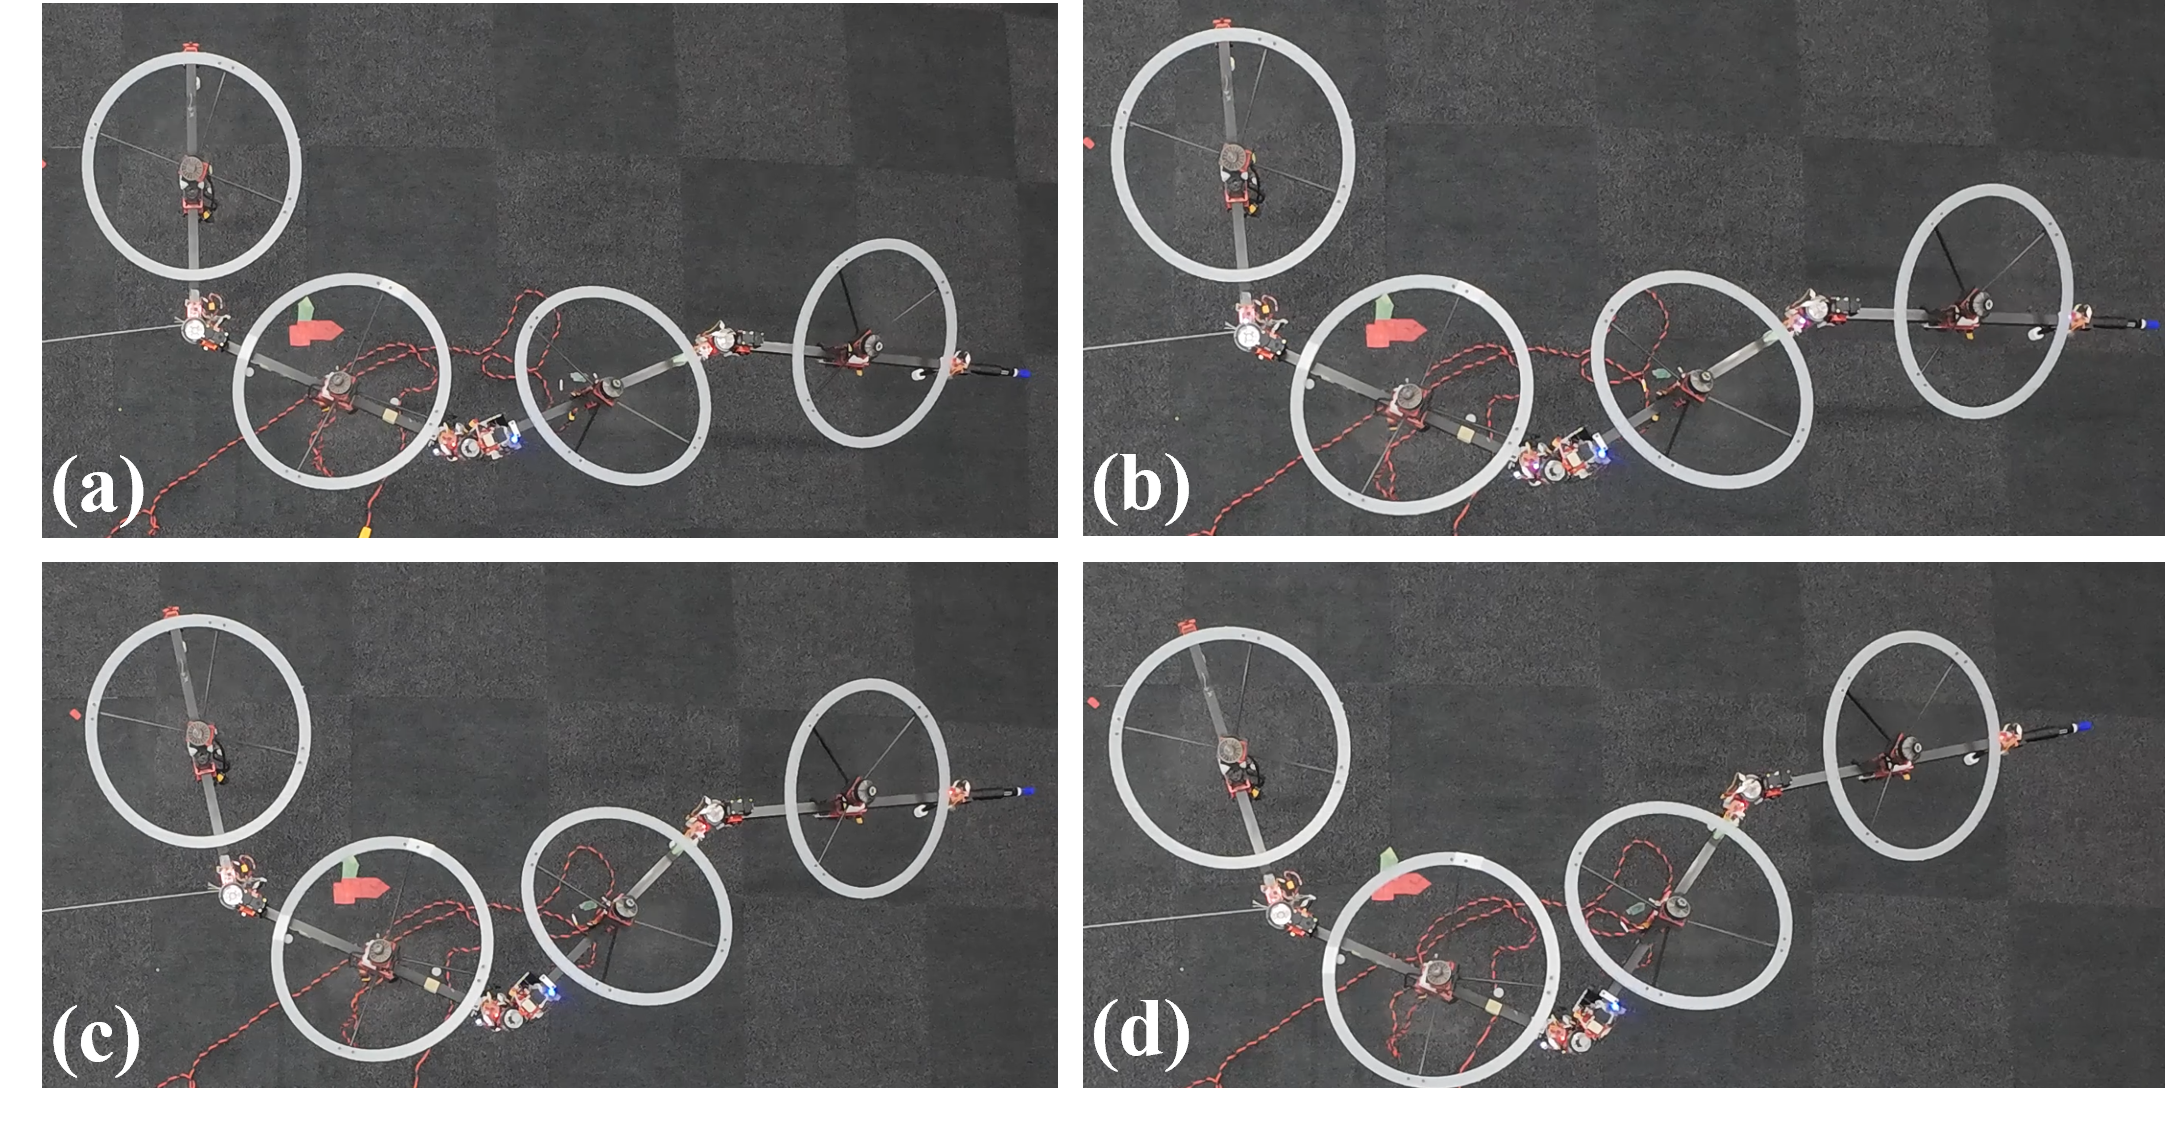
\includegraphics[trim={0cm 0.3cm 0cm 0cm},clip,width=\linewidth]{figures/chapter3/admittance_changing.png}
    \caption{Admittance changing.}
    \label{fig:admittance_changing}
    \vspace{-5mm}
\end{figure}

\subsection{Hybrid Control Mechanism} 

In surface-sliding tasks with the secondary requirements. As illustrated in Fig.~\ref{fig:hybrid_controller}, impedance control is applied for adjusting the distance between the prior frame and the prior trajectory, and the admittance control is applied for adjusting the distance between the secondary frame and the secondary trajectory.


\begin{figure}[h]
    \centering
    % \parbox{3in}
    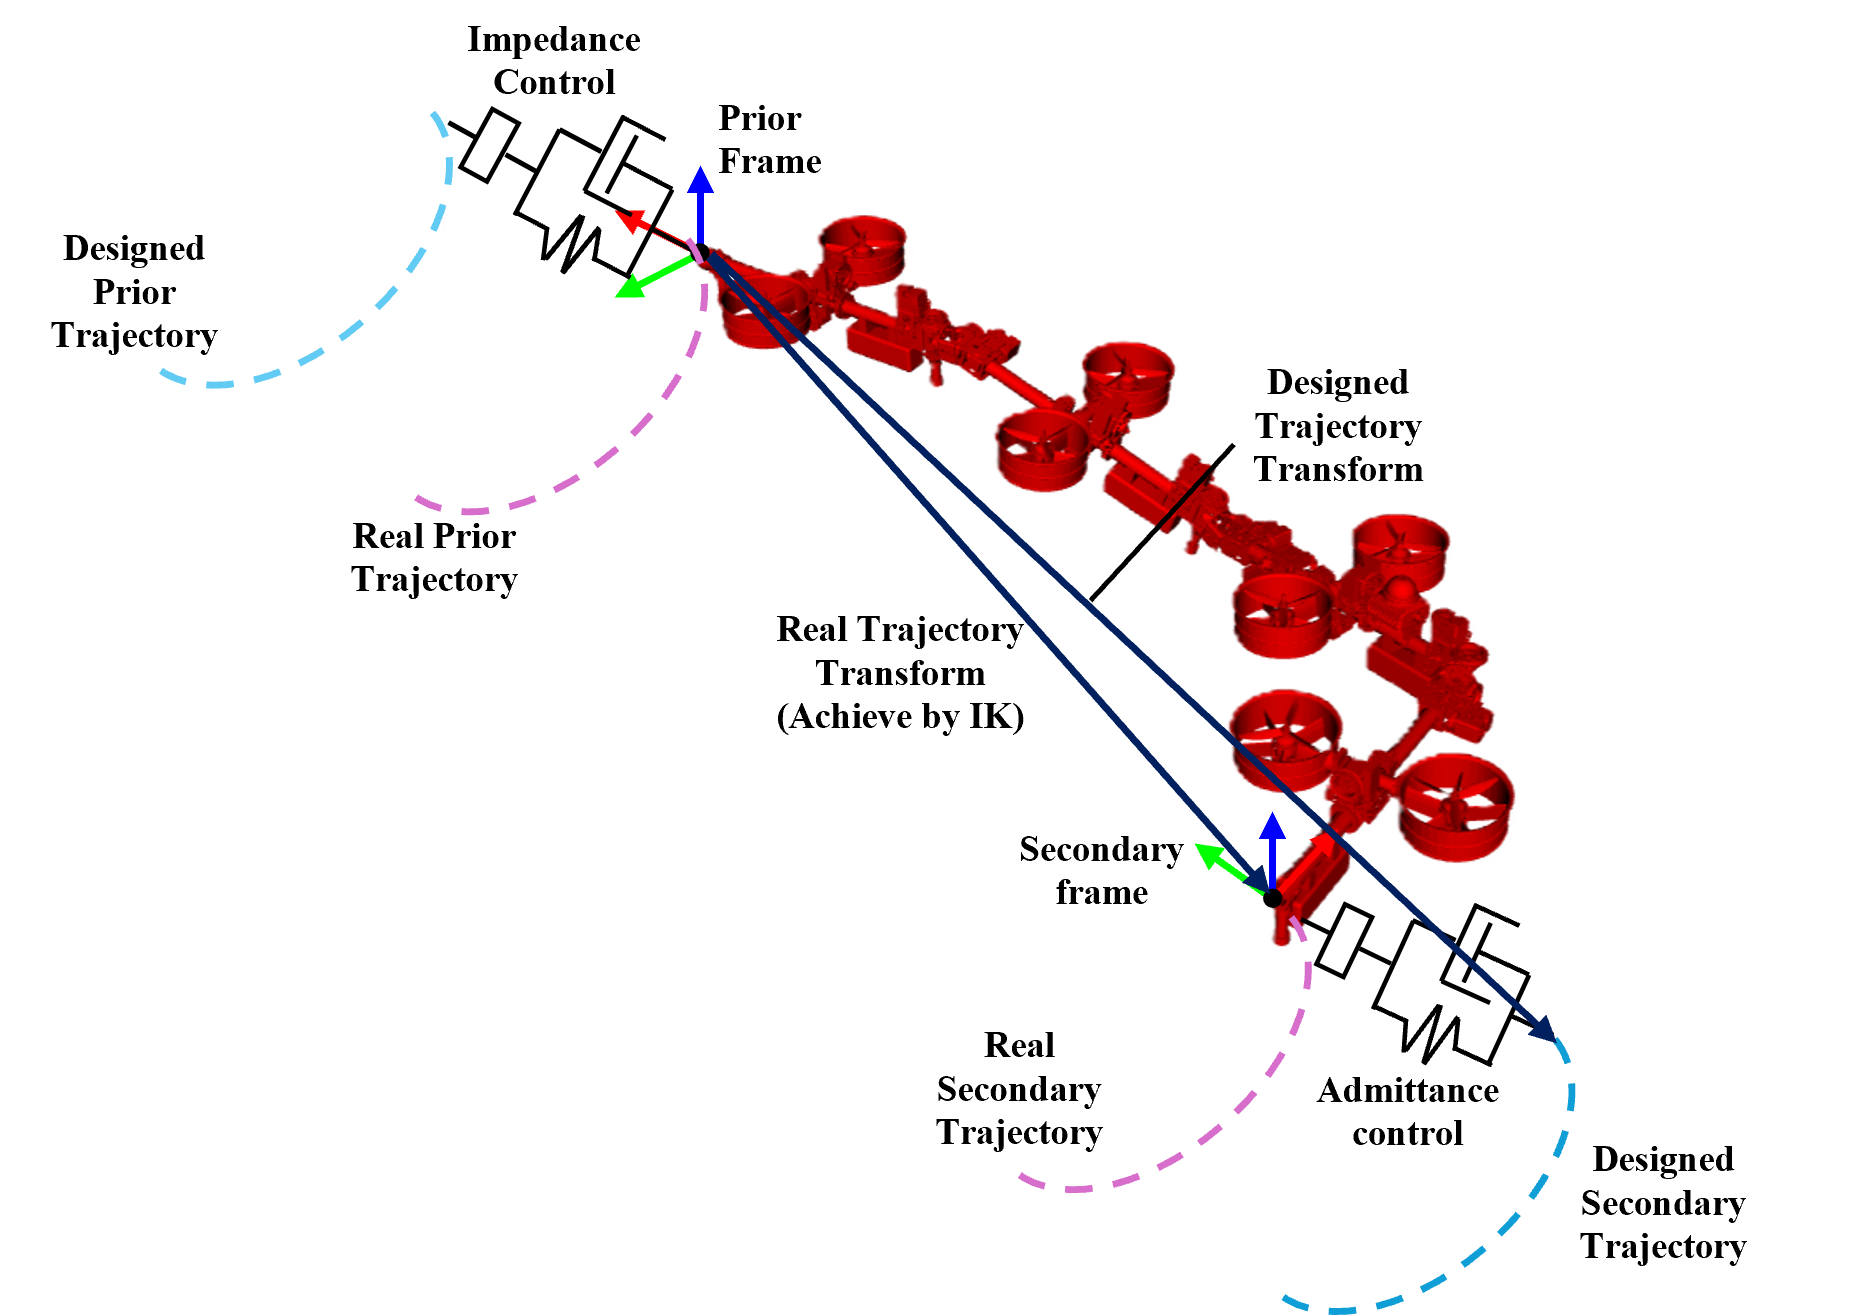
\includegraphics[trim={0cm 0.3cm 0cm 0cm},clip,width=\linewidth]{figures/chapter4/dragon_hybrid.png}
    \caption{Schematic diagram of the hybrid impedance-admittance control.}
    \label{fig:dragon_hybrid}
    \vspace{-5mm}
\end{figure}

% the contact and sliding directions exhibit fundamentally different physical characteristics: the sliding directions are dominated by friction-induced disturbances, whereas the contact direction is shaped by geometric variations of the environment. Leveraging this distinction, the hybrid impedance–admittance controller assigns each axis the control behavior best suited to its interaction properties. As illustrated in Fig.~\ref{fig:hybrid_controller}, admittance control is applied along the contact direction ($x$ axis) to regulate geometry-driven variations, while impedance control governs the sliding directions ($y$ and $z$ axes) to accommodate friction-affected motion.

% Through this task-aligned division of control responsibilities, the hybrid controller achieves what neither controller can provide alone: robust sliding performance in the sliding directions and adaptive behavior in the contact direction. This directional decomposition is enabled by the actuation structure of the multi-link aerial robot, which allows the two control paradigms to be realized simultaneously through independent actuation sources. This combination is therefore essential for achieving resilient interaction and adaptive contact behavior in surface-sliding tasks. The performance of the proposed hybrid impedance-admittance controller will be exhibited in the experiment chapter.
% %%%%%%%%%%%%%%%%%%%%%%%%%%%%%%%%%%%%%%%%%%%%%%%%%%%%%%%%%%%%%%%%%%%%%%%%%%%%%%%%
% \section{Experimental Validation}
% \subsection{Impedance control}
% \subsection{Inverse Kinematics}
% \subsection{Admittance control}
%%%%%%%%%%%%%%%%%%%%%%%%%%%%%%%%%%%%%%%%%%%%%%%%%%%%%%%%%%%%%%%%%%%%%%%%%%%%%%%%
\section{Summary}
In this chapter, we realize the hybrid control of dragon. We first discuss the necessity of using the hybrid control. We express the different impedance control mode. Finally use it in the dragon. Transparently, the kind of control method can be promoted to solve more complicated aerial manipulation tasks.